
\setchapterpreamble[u]{\margintoc}
\chapter{Multiple potentials}

Until this moment we have only work with 1 potential well but if our goal is to understand solids and their properties we need to figure out how our quantum world works with multiple potential.


\section{Definition}

\begin{marginfigure}
  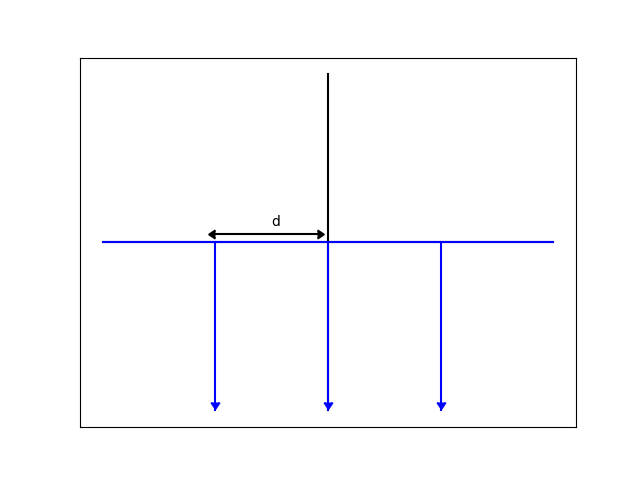
\includegraphics{images5/def.png}
  \centering
  \caption{Multiple delta function potentials problem.}
  \labfig{fig_5.1}
\end{marginfigure}

In this problem we will have N delta function potentials, as the one in the previous chapter, separated by a distance d, with a fix value for g of g=1. The potential can be defined as:

\begin{equation}
  \label{5.1}
  "V(x) = -2 V_0 a \left[\sum_{n=1}^{N} \delta(x-nd) \right]"
\end{equation}

Using \ref{5.1} we get the wave equation for this problem.

\begin{equation}
  \label{5.2}
  "\alpha^2\phi(x) = \frac{\partial^2\phi(x)}{\partial x^2} + 2 g \left[\sum_{n=1}^{N} \delta(x-nd) \right] \phi(x)"
\end{equation}

Outside of the potentials the equation to solve will be the same as \ref{4.6}, our goal is going to be trying to find the relation between the A and B coefficients at both sides of a potential as we can see in \reffig{fig_5.2}

\begin{figure}[H]
  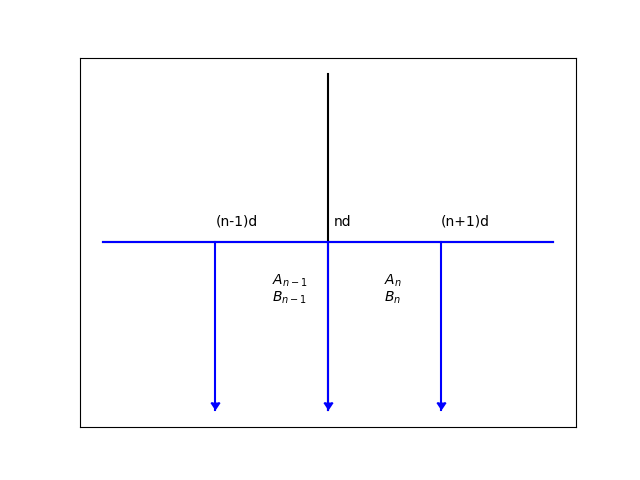
\includegraphics{images5/def_n.png}
  \centering
  \caption{Coefficients outside of the potentials near x=nd.}
  \labfig{fig_5.2}
\end{figure}

\section{Solution}

Our potential at $x=nd$ will look like \reffig{fig_5.2} and the solution at the left and right side of the potential in x=nd will be: \marginnote[2pt]{We are adding the term $ -nd\pm d/2$ in the exponential because it will make the math easier later.}


\begin{equation}
  \label{5.3}
  \begin{array}{lc}
    \phi(x) = A_{n-1}e^{-\alpha(x-[nd-\frac{d}{2}])}+B_{n-1}e^{\alpha(x-[nd-\frac{d}{2}])} & x < nd
    \\

    \\
    \phi(x) = A_{n}e^{-\alpha(x-[nd+\frac{d}{2}])}+B_{n}e^{\alpha(x-[nd+\frac{d}{2}])} & x > nd
  \end{array}
\end{equation}



First, if we look at the limits when n=1 and n=N we get the solutions from the previous chapter.

\begin{equation}
  \label{5.4}
  \begin{array}{l}
    A_0 = 0 \\
    B_N = 0
  \end{array}
\end{equation}

We will use the continuity of the function and its derivatives, as we already explain in Chapter 4, to relate the A and B coefficients.

The first condition is that $\phi(x)$ is continuous. To simplify we will use $v = e^{-\alpha\frac{d}{2}}$.

\begin{equation}
  \label{5.5}
  A_{n-1}v+\frac{B_{n-1}}{v} = \frac{A_n}{v}+B_n v
\end{equation}

The second condition is our relation between the derivatives in $x=nd$ shown in \ref{4.11}

\begin{equation}
  \label{5.6}
  \begin{array}{l}
    [-\alpha A_{n-1} v + \alpha \frac{B_{n-1}}{v}]-[-\alpha\frac{A_n}{v}+\alpha B_n v] = 2[A_{n-1}v+\frac{B_{n-1}}{v}]
    \\

    \\
    A_{n-1}(-\alpha v-2v)+B_{n-1}(\frac{\alpha}{v}-\frac{2}{v}) = -\alpha A_n \frac{1}{v}+\alpha B_n v
    \\

    \\
    -A_n\frac{1}{v} + B_n v = -vA_{n-1}(1+\frac{2}{\alpha})+\frac{1}{v}B_{n-1}(1-\frac{2}{\alpha})
  \end{array}
\end{equation}

If we add and substract both conditions we will get the next equations:

\begin{equation}
  \label{5.7}
  \begin{array}{l}
    B_n = -\frac{1}{\alpha} A_{n-1} + \frac{1}{v^2}(1-\frac{1}{\alpha}) B_{n-1}
    \\

    \\
    A_n = v^2(1+\frac{1}{\alpha})A_{n-1} + \frac{1}{\alpha} B_{n-1}
  \end{array}
\end{equation}

We want to show this like a matrix.

\begin{equation}
  \label{5.8}
  \left(\begin{array}{c}
    A_n
    \\

    \\
    B_n
  \end{array}
  \right) =
  \left[
    \begin{array}{cc}
      v^2(1+\frac{1}{\alpha}) & \frac{1}{\alpha}
      \\

      \\
      -\frac{1}{v} & \frac{1}{v^2}(1-\frac{1}{\alpha})
    \end{array}
  \right]
  \left(\begin{array}{c}
    A_{n-1}
    \\

    \\
    B_{n-1}
  \end{array}
  \right)
\end{equation}

We will called this matrix T. Now we can relate any index with each other because T does not depend on n, i.e. $T = T(\alpha,d)$. Now we will find the solutions for alpha using the relation between n=1 and n=N coefficients.

\begin{equation}
  \label{5.9}
  \left(\begin{array}{c}
    A_N
    \\

    \\
    B_N
  \end{array}
  \right) =
  \left[
    T
  \right]^N
  \left(\begin{array}{c}
    A_{0}
    \\

    \\
    B_{0}
  \end{array}
  \right)
\end{equation}

To solve for alpha we will use \ref{5.4}.

\begin{equation}
  \label{5.10}
  \left(\begin{array}{c}
    A_N
    \\

    \\
    0
  \end{array}
  \right) =
  \left[
    \begin{array}{cc}
      (T^N)_{11} & (T^N)_{12}
      \\

      \\
      (T^N)_{21} & (T^N)_{22}
    \end{array}
  \right]
  \left(\begin{array}{c}
    0
    \\

    \\
    B_{0}
  \end{array}
  \right)
\end{equation}

For this equations to be true we get the condition, $(T^N)_{22}=0$. This will give the solutions for alpha and will depend only on d. \marginnote[2pt]{However, the number of solutions for alpha will be dependent on N, i.e. the number of delta function potentials}


\section{Solutions for N = 1,2}

Now that we have the general solution, we can try to get the simplest examples.

For N = 1 it will be extremely simple.

\begin{equation}
  \label{5.11}
  \frac{1}{v^2}(1-\frac{1}{\alpha}) = 0
\end{equation}

Solving for $\alpha$ we get $\alpha=1$ that exactly the value for g, this tell us that when N=1 we recover the solution from the previous chapter, wich make sense.

For N = 2 we need to square the matrix.

\begin{equation}
  \label{5.12}
  \begin{array}{c}
    T^2 = \left[
      \begin{array}{cc}
        v^2(1+\frac{1}{\alpha}) & \frac{1}{\alpha}
        \\

        \\
        -\frac{1}{\alpha} & \frac{1}{v^2}(1-\frac{1}{\alpha})
      \end{array}
    \right]^2=

    \\

    \\

    =\left[
      \begin{array}{cc}
        v^2(1+\frac{1}{\alpha}) & \frac{1}{\alpha}
        \\

        \\
        -\frac{1}{\alpha} & \frac{1}{v^2}(1-\frac{1}{\alpha})
      \end{array}
    \right]
    \left[
      \begin{array}{cc}
        v^2(1+\frac{1}{\alpha}) & \frac{1}{\alpha}
        \\

        \\
        -\frac{1}{\alpha} & \frac{1}{v^2}(1-\frac{1}{\alpha})
      \end{array}
    \right] =

    \\

    \\

    =
    \left[
      \begin{array}{cc}
        v^4(1+\frac{1}{\alpha})^2-\frac{1}{\alpha^2} & \frac{1}{\alpha}[v^2(1+\frac{1}{\alpha})+\frac{1}{v}(1-\frac{1}{\alpha})]
        \\

        \\
        -\frac{1}{\alpha}[v^2(1+\frac{1}{\alpha})+\frac{1}{v}(1-\frac{1}{\alpha})] & -\frac{1}{\alpha^2} + \frac{1}{v^4}(1-\frac{1}{\alpha})^2
      \end{array}
    \right]
  \end{array}
\end{equation}

From the expresion of $T_{22}$ we can get the solutions for alpha.

\begin{equation}
  \label{5.13}
  \begin{array}{c}
    -\frac{1}{\alpha^2} + \frac{1}{v^4}(1-\frac{1}{\alpha})^2 = 0 \\
    \pm \frac{1}{\alpha} = e^{\alpha d}(1-\frac{1}{\alpha})
  \end{array}
\end{equation}

We get two different solutions from this equation.

\begin{equation}
  \label{5.14}
  \begin{array}{c}
    \alpha = 1 + e^{-\alpha d}

    \\

    \alpha = 1 - e^{-\alpha d}
  \end{array}
\end{equation}

\begin{marginfigure}
  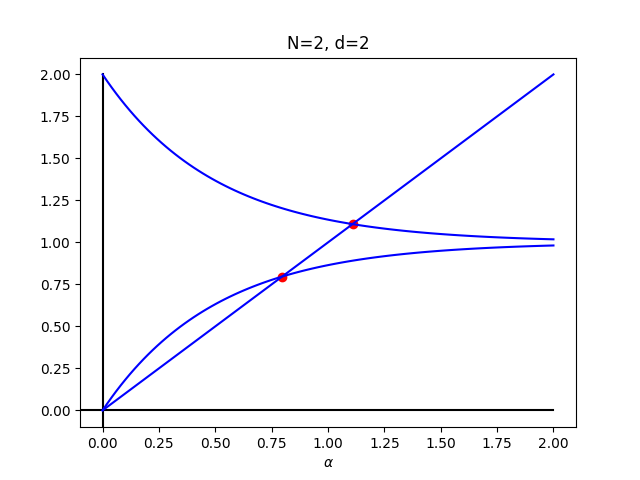
\includegraphics{images5/N=2,d=2.png}
  \centering
  \caption{Solutions for $(T^N)_{22} = 0$ for N=2 and d=2}
  \labfig{fig_5.3}
\end{marginfigure}

If we plot both sides of the equations we can see two different results depending on d. If d is greater than 1 we will get two solutions if d is least than 1 we will only find one solution. This can be observe in \reffig{fig_5.3} and \reffig{fig_5.4}. \marginnote{The solutions have been found using numerical analysis.}

\begin{marginfigure}
  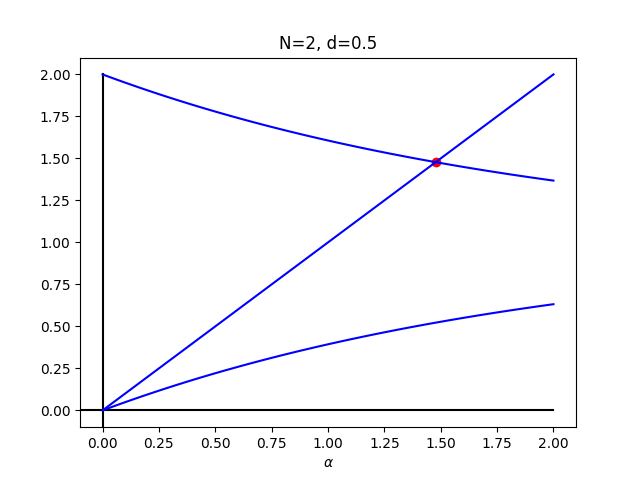
\includegraphics{images5/N=2,d=0.5.png}
  \centering
  \caption{Solutions for $(T^N)_{22} = 0$ for N=2 and d=0.5}
  \labfig{fig_5.4}
\end{marginfigure}


\begin{figure}
  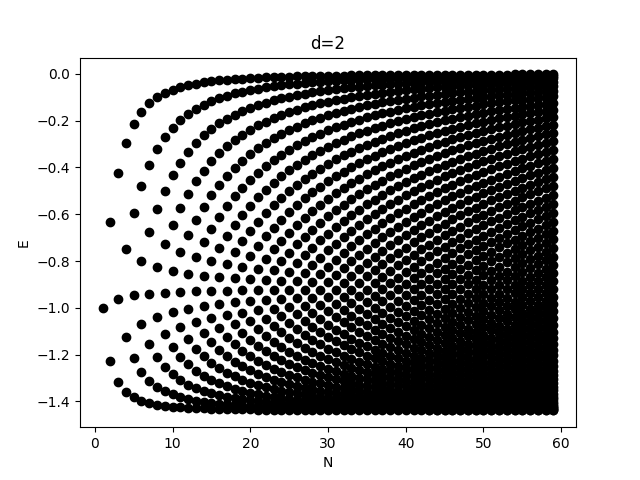
\includegraphics[H]{images5/N_E_d_eff=2.png}
  \centering
  \caption{alpha as a function of N for $d = 2$.}
  \labfig{fig_5.5}
\end{figure}

As N increase with a fix d the number of alphas will increase until the discrete turns into a almost continuous behaviour. For an infinite N we will aproach a continuous energy range with posible energies. With N from 1 to 60 we can see the behaviour of the energy when d=2 and we can appreciate how the posible energies are more and more continuous for larger N.


\section{Solving for x as a circunference}

If we assume x axis is not a straight line, and instead it is inside a circunference of length L, like \reffig{fig_5.6}, the math will look better and we will get some interesting new results.

\begin{marginfigure}
  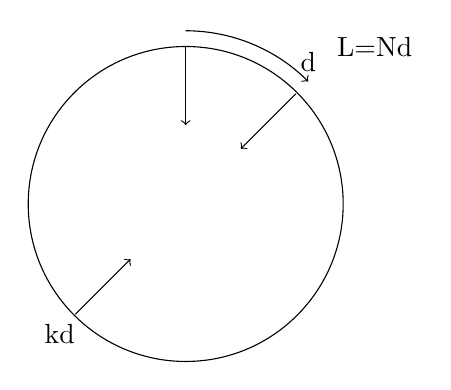
\begin{tikzpicture}

    \draw[black] (0,0) circle (2);
    \draw[->] (0,2) -- (0,1);
    \draw[->] (1.4,1.4) -- (0.7,0.7);
    \draw[->] (-1.4,-1.4) -- (-0.7,-0.7);
    \filldraw[black] (-1.6,-1.4) circle (0) node [anchor=north]{kd};
    \filldraw[black] (3,2) circle (0) node [anchor=east]{L=Nd};
    \draw[->] (0,2.2) arc (90:45:2.2) node[anchor=south]{d};
    \end{tikzpicture}
    \caption[x as a circunference]{x as a circunference of distance L.}
    \labfig{fig_5.6}
\end{marginfigure}

Because we have N potentials separated a distance d, we can say that $L= Nd$. When N is infinite we will have again that L is aproximately infinite and therefore the circunference will recover the straight line shape.

One of the consequences of this new aproach is that now E is not confined to only negative values. We know get a new wave equation where E is the energy.

\begin{equation}
  \label{5.15}
  -\frac{\hbar^2}{2m}\frac{d^2\phi}{dx^2} + V(x)\phi(x) = E\phi(x)
\end{equation}

We have to solve this equation with our boundaries as before, but we have new boundaries as a result of our transformation. We can use the rotation simetry to say that now our function is periodic. This give us new conditions:


\begin{equation}
  \label{5.16}
  \begin{array}{c}
    \phi(x+L) = \phi(x)

    \\

    \frac{d\phi}{dx}(x+L) = \frac{d\phi}{dx}(x)

    \\

    V(x+L) = V(x)
  \end{array}
\end{equation}

We want to go even further and solve problems where $V(x)$ is periodic in d instead of L, i.e. $V(x+d)=V(x)$.

In this case we say, and it can be prove, that $\phi(x)$ is quasi-periodic.

\begin{equation}
  \label{5.17}
  \phi(x+d) = C \phi(x)
\end{equation}

After the N potentials $\phi(x)$ must be the same again according to \ref{5.16}.

\begin{equation}
  \label{5.18}
  \phi(x+Nd) = C^N \phi(x) = \phi(x+L) = \phi(x)
\end{equation}

This means that $C^N = 1$ and this lead us to N solutions for C.

\begin{equation}
  \label{5.19}
  \begin{array}{lc}
    C = e^{i\frac{2\pi}{N}k} & k=0,1,2,...,N-1
  \end{array}
\end{equation}

We will solve the problem between d/2 and -d/2 as we can see in \reffig{fig_5.7}

\begin{marginfigure}
  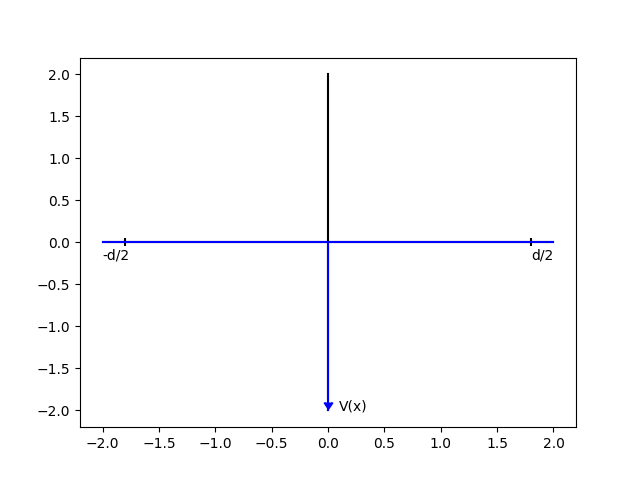
\includegraphics{images5/quasiperf.png}
  \centering
  \caption{Potential between -d/2 and d/2}
  \labfig{fig_5.7}
\end{marginfigure}

Outside of the potential the wave equation is:

\begin{equation}
  \label{5.20}
  \frac{d^2\phi(x)}{dx^2} =
  \left\{
  \begin{array}{lc}
    \alpha^2 \phi(x) & E < 0
    \\
    \beta^2  \phi(x) & E > 0
  \end{array}
  \right.
\end{equation}

The solution fo this equations is the same as the one in Chapter 4, but we will change the notation, intead of terms of n we will called the coefficients $A_L$, $B_L$ and $A_R$, $B_R$, for left and right of the potential.

Let's resume all the conditions.

\begin{equation}
  \label{5.21}
  \begin{array}{lc}
    I) & \phi(d/2) = C \phi(-d/2)

    \\

    \\

    II) & \frac{\phi}{dx}(d/2) = C \frac{\phi}{dx}(-d/2)

    \\

    \\

    III) & \phi(x=0^{-}) = \phi(x=0^{+})

    \\

    \\

    IV) & \left.\frac{d\phi}{dx}\right|_{x=0^{-}} - \left.\frac{d\phi}{dx}\right|_{x=0^{+}} = 2\phi(0)
  \end{array}
\end{equation}

We have to solve for this conditions. We will use $v = e^{d\alpha/2}$ to simplify the math.


\begin{equation}
  \label{5.22}
  \begin{array}{lc}

    I + II & B_R = \frac{C}{v^2} B_L

    \\

    \\

    I-II & A_R = C v^2 A_L

    \\

    \\

    III => & (Cv^2-1) A_L = (1-\frac{C}{v^2}) B_L

    \\

    \\

    IV => & [-A_L\alpha+B_L\alpha] - [-A_R\alpha + B_R\alpha] = 2[A_L + B_L]
  \end{array}
\end{equation}

Combining the four expresions we can get the equation to solve alpha for.

\begin{equation}
  \label{5.23}
  \cos{\left(\frac{2\pi k}{N}\right)} = \cosh{(\alpha d)} - \frac{1}{\alpha} \sinh{(\alpha d)}
\end{equation}

If d and N are given we can get $\alpha(k)$.

To see the behaviour of the function with N we can fixed d and try to get all the solutions for alpha. We can see in \reffig{fig_5.8} how the energy range became continuous when N increase to infinite.

\begin{figure}[H]
  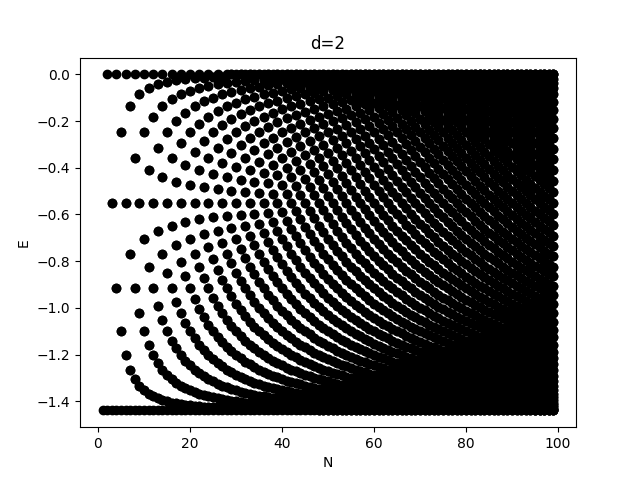
\includegraphics{images5/E_d=2_N.png}
  \centering
  \caption{Energy as a function of the number of potentials.}
  \labfig{fig_5.8}
\end{figure}

In the other hand, if we want to see the behaviour of the function with d, we have to do before a numerical analisis of the function in the right side. First, we want to find the limit for $\alpha \to 0$. We will need to use Taylor expansion to solve it.

\begin{equation}
  \label{5.24}
  \begin{array}{c}
    \lim_{\alpha \to 0} (\cosh{(\alpha d)} - \frac{1}{\alpha} \sinh{(\alpha d)}) =
    \\

    \\
    = \cosh{(0)} - \lim_{\alpha \to 0} \frac{1}{\alpha} \frac{e^{\alpha d}-e^{-\alpha d}}{2} =
    \\

    \\
    = 1 - \lim_{\alpha \to 0} \frac{1}{\alpha} \frac{2\alpha d + o(\alpha^2)}{2} = 1-d
  \end{array}
\end{equation}

Now we want to see how the monotony of the function behaves, so we have to look at the derivative of the function. We will use taylor expansion again.


\begin{equation}
  \label{5.25}
  \begin{array}{c}
    \frac{d}{dx}\left[\cosh{(\alpha d)} - \frac{1}{\alpha} \sinh{(\alpha d)} \right] =
    \\

    \\
    = \left(\alpha + \frac{1}{\alpha^2}\right)\sinh{(\alpha d)} -\frac{d}{\alpha}\cosh{(\alpha d)} \approx
    \\

    \\
    \approx \alpha d^2 (1-\frac{d}{3}) + o(\alpha^3)
  \end{array}
\end{equation}

If d is greater than 3 the function decreases first and then it increases until infinity. If d is less than 3 the function increases for all $\alpha$. Is not important for us where the minimum is located, the key aspect is that if d is greater than 3 we get solutions for bigger alphas of the equation because the left function is confine in [-1,1].

In \reffig{fig_5.9} we can see that for a fixed value of N we can get all the energies depending on the distance. If we take a look into the maximum energy we can see that for values of d greater than 2, this value starts to decrease.

\begin{figure}[H]
  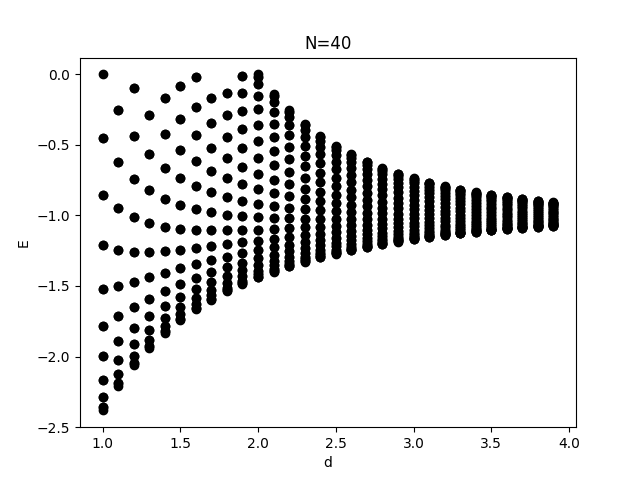
\includegraphics{images5/E_d_N=40.png}
  \centering
  \caption{Energy as a function of the distance between potentials.}
  \labfig{fig_5.9}
\end{figure}

\section{Solution for all the posible energies.}

This is not the end of the chapter because as we already said, we have also positive energies. Solving for the second equation in \ref{5.20} we get a similar equation to \ref{5.23} but where $\beta = i\alpha$.

\begin{equation}
  \label{5.26}
  \cos{\left(\frac{2\pi k}{N}\right)} = \cos{(\beta d)} - \frac{1}{\beta} \sinh{(\beta d)}
\end{equation}

Plotting all the solutions together, the positive and the negative ones, we can see how the energy levels behaves depending on the other two parameters, d and N. Moreover we can also see the gaps between the different energy levels.

\begin{figure}[H]
  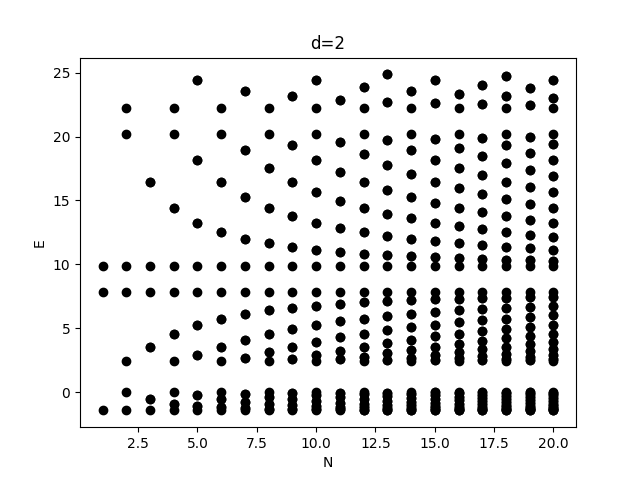
\includegraphics{images5/Etotal_d=2_N.png}
  \centering
  \caption{All the energies as a function of the number of potentials.}
  \labfig{fig_5.10}
\end{figure}

\begin{figure}[H]
  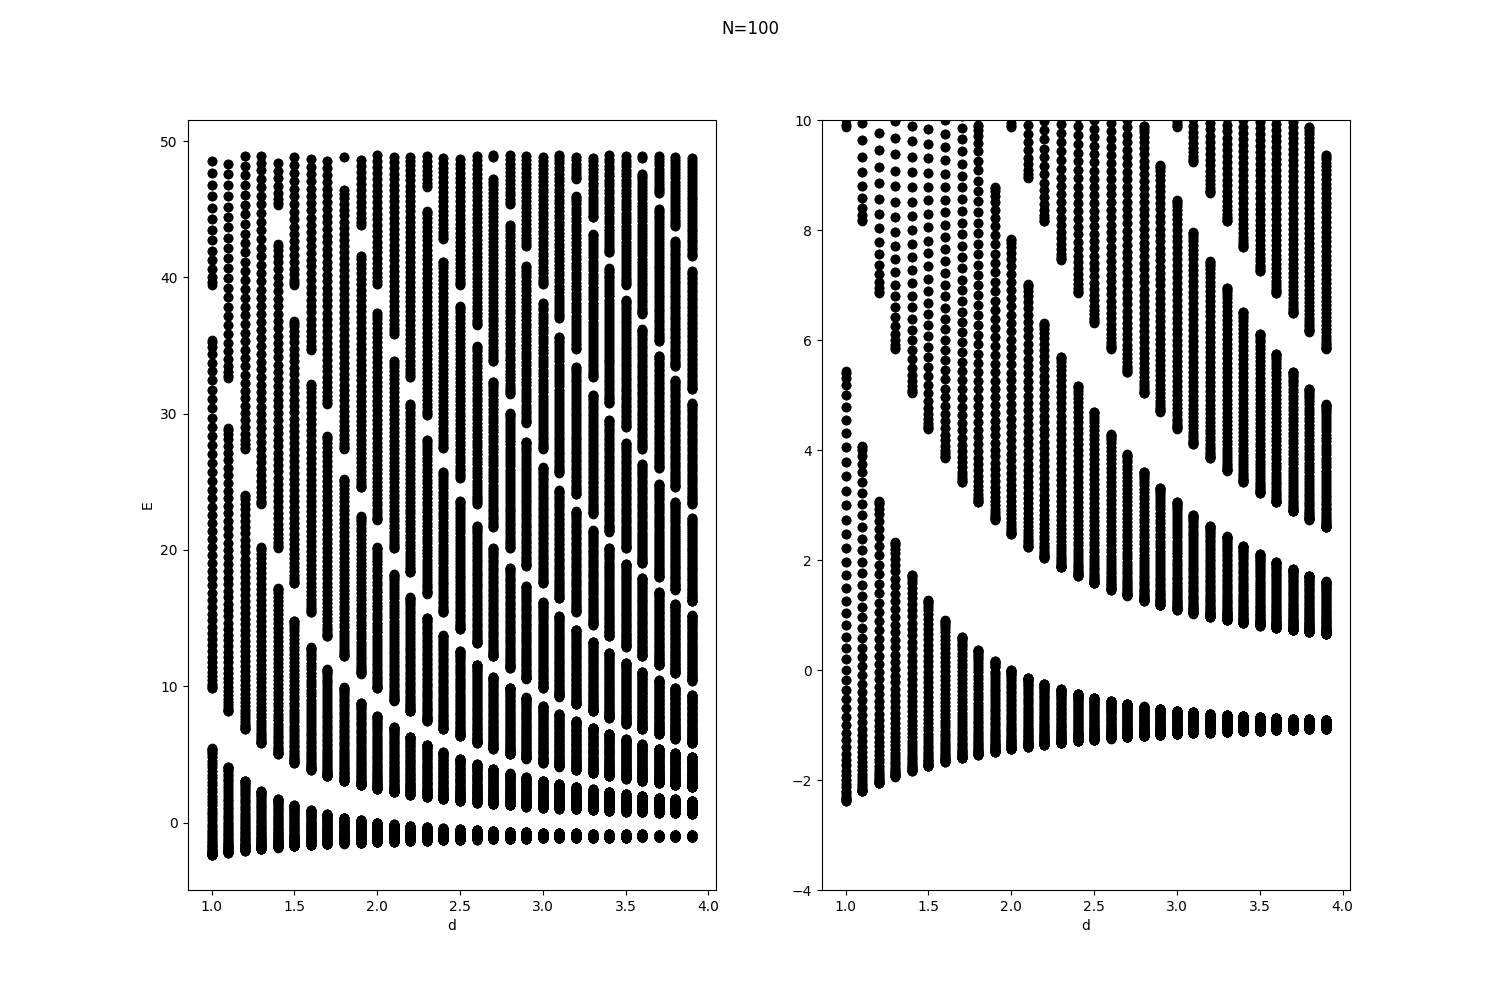
\includegraphics{images5/Etotal_d_N=100.png}
  \centering
  \caption{All the energies as a function of the distance between potentials.}
  \labfig{fig_5.11}
\end{figure}

In the figures above is appreciated how the energy levels are well define and the distance between them remain constant when we increase N.However while d goes to ifinite the width of the energy levels is decreasing.

There are more complicated problems that could be solved using this way of thinking. In this book we proposed the reader to solve this problem adding a new parameter, a, that is the distance between two potentials. Where d is still quasiperiodic and is the distance between this two pairs and the next pair.

% \setchapterimage[6cm]{seaside}
% \setchapterpreamble[u]{\margintoc}
% \chapter{Page Design}
% \labch{layout}

% \section{Headings}

% So far, in this document I used two different styles for the chapter
% headings: one has the chapter name, a rule and, in the margin, the
% chapter number; the other has an image at the top of the page, and the
% chapter title is printed in a box (like for this chapter). There is one
% additional style, which I used only in the \nrefch{appendix}; there, the chapter title is enclosed in two
% horizontal rules, and the chapter number (or letter, in the case of the
% appendix) is above it.\sidenote{To be honest, I do not think that mixing
% heading styles like this is a wise choice, but in this document I did it
% only to show you how they look.}

% Every book is unique, so it makes sense to have different styles from
% which to choose. Actually, it would be awesome if whenever a
% \Class{kao}-user designs a new heading style, he or she added it to the
% three styles already present, so that it will be available for new users
% and new books.

% The choice of the style is made simple by the \Command{setchapterstyle}
% command. It accepts one option, the name of the style, which can be:
% \enquote{plain}, \enquote{kao}, \enquote{bar}, or
% \enquote{lines}.\sidenote{Plain is the default \LaTeX\xspace title
% style; the other ones are self explanatory.} If instead you want the
% image style, you have to use the command \Command{setchapterimage},
% which accepts the path to the image as argument; you can also provide an
% optional parameter in square brackets to specify the height of the
% image. \Command{setchapterimage} automatically sets the chapter style to
% \enquote{bar} for that chapter (and also for subsequent chapters).

% Let us make some examples. In this book, I begin a normal chapter with
% the lines:
% \begin{lstlisting}
% \setchapterstyle{kao}
% \setchapterpreamble[u]{\margintoc}
% \chapter{Title of the Chapter}
% \labch{title}
% \end{lstlisting}

% In Line 1 I choose the style for the title to be \enquote{kao}. Then, I
% specify that I want the margin toc. The rest is ordinary administration
% in \LaTeX, except that I use my own \Command{labch} to label the
% chapter. Actually, the \Command{setchapterpreamble} is a standard
% \KOMAScript\xspace one, so I invite you to read about it in the KOMA
% documentation. Once the chapter style is set, it holds until you change
% it.\sidenote{The \Command{margintoc} has to be specified at every
% chapter. Perhaps in the future this may change; it all depends on how
% this feature will be welcomed by the users, so keep in touch with me if
% you have preferences!} Whenever I want to start a chapter with an image,
% I simply write:

% \begin{lstlisting}
% \setchapterimage[7cm]{path/to/image.png} % Optionally specify the height
% \setchapterpreamble[u]{\margintoc}
% \chapter{Catchy Title} % No need to set a chapter style
% \labch{catchy}
% \end{lstlisting}

% If you prefer, you can also specify the style at the beginning of the
% main document, and that style will hold until you change it again.

% \section{Headers \& Footers}

% Headers and footers in \KOMAScript\xspace are handled by the
% \Package{scrlayer-scrpage} package. There are two basic style:
% \enquote{scrheadings} and \enquote{plain.scrheadings}. The former is
% used for normal pages, whereas the latter is used in title pages (those
% where a new chapter starts, for instance) and, at least in this book, in
% the front matter. At any rate, the style can be changed with the
% \Command{pagestyle} command, \eg
% \lstinline|\pagestyle{plain.scrheadings}|.

% In both styles, the footer is completely empty. In plain.scrheadings,
% also the header is absent (otherwise it wouldn't be so plain\ldots), but
% in the normal style the design is reminiscent of the \enquote{kao} style
% for chapter titles.

% \begin{kaobox}[frametitle=To Do]
% The \Option{twoside} class option is still unstable and may lead to
% unexpected behaviours. As always, any help will be greatly appreciated.
% \end{kaobox}

% \section{Table of Contents}

% Another important part of a book is the table of contents. By default,
% in \Class{kaobook} there is an entry for everything: list of figures,
% list of tables, bibliographies, and even the table of contents itself.
% Not everybody might like this, so we will provide a description of the
% changes you need to do in order to enable or disable each of these
% entries. In the following \reftab{tocentries}, each item corresponds to
% a possible entry in the \acrshort{tocLabel}, and its description is the
% command you need to provide to have such entry. These commands are
% specified in the attached \href{style/style.sty}{style
% package},\sidenote{In the same file, you can also choose the titles of
% these entries.} so if you don't want the entries, just comment the
% corresponding lines.

% Of course, some packages, like those for glossaries and indices, will
% try to add their own entries.\marginnote{In a later section, we will see
% how you can define your own floating environment, and endow it with an
% entry in the \acrshort{tocLabel}.} In such cases, you have to follow the
% instructions specific to that package. Here, since we have talked about
% glossaries and notations in \refch{references}, we will briefly see how
% to configure them.

% \begin{table}
% \footnotesize
% \caption{Commands to add a particular entry to the table of contents.}
% \labtab{tocentries}
% \begin{tabular}{ l l }
% 	\toprule
% 	Entry & Command to Activate \\
% 	\midrule
% 	Table of Contents & \lstinline|\setuptoc{toc}{totoc}| \\
% 	List of Figs and Tabs & \lstinline|\PassOptionsToClass{toc=listof}{\@baseclass}| \\
% 	Bibliography & \lstinline|\PassOptionsToClass{toc=bibliography}{\@baseclass}| \\
% 	\bottomrule
% \end{tabular}
% \end{table}

% For the \Package{glossaries} package, use the \enquote{toc} option when
% you load it: \lstinline|\usepackage[toc]{glossaries}|. For
% \Package{nomencl}, pass the \enquote{intoc} option at the moment of
% loading the package. Both \Package{glossaries} and \Package{nomencl} are
% loaded in the attached \href{style/packages.sty}{\enquote{packages}
% package}.

% Additional configuration of the table of contents can be performed
% through the packages \Package{etoc}, which is loaded because it is
% needed for the margintocs, or the more traditional \Package{tocbase}.
% Read the respective documentations if you want to be able to change the
% default \acrshort{tocLabel} style.\sidenote[][*-1]{(And please, send me
% a copy of what you have done, I'm so curious!)}

% \section{Paper Size}

% Recent versions of Kaobook support paper sizes different from the
% default A4. It is possible to pass the name of the paper as an option
% to the class, as we are accustomed for any other \LaTeX\ class. For
% example, the class option \Option{b5paper} would set the paper size
% to the B5 format.

% We also support the paper sizes specified in
% \href{https://www.bod.de/hilfe/hilfe-und-service.html?cmd=SINGLE\&entryID=2494\_GER\_WSS\&eo=2\&title=welche-buchformate-gibt-es}{this
% web page} and some additional sizes requested by the users, with the
% option names specified in \reftab{papersizes}.

% \begin{margintable}[*-6]
% 	\caption{Some non-standard paper sizes supported by kaobook.}
% 	\labtab{papersizes}
% 	\begin{tabular}{ll}
% 		\toprule
% 		Dimension & Option name \\
% 		\midrule
% 		12.0cm x 19.0cm & smallpocketpaper \\
% 		13.5cm x 21.5cm & pocketpaper \\
% 		14.8cm x 21.0cm & a5paper \\
% 		15.5cm x 22.0cm & juvenilepaper \\
% 		17.0cm x 17.0cm & smallphotopaper \\
% 		21.0cm x 15.0cm & appendixpaper \\
% 		17.0cm x 22.0cm & cookpaper \\
% 		19.0cm x 27.0cm & illustratedpaper \\
% 		17.0cm x 17.0cm & photopaper \\
% 		16.0cm x 24.0cm & f24paper \\
% 		%21.0cm x 29.7cm & a4paper \\
% 		\bottomrule
% 	\end{tabular}
% \end{margintable}

% For instance, to use the \enquote{smallpocketpaper} add the correct
% description at the beginning of the documentclass instruction:
% \begin{lstlisting}
% \documentclass[
% 		smallpocketpaper,
% 		fontsize=10pt,
% 		twoside=false,
% 		%open=any,
% 		secnumdepth=1,
% ]{kaobook}
% \end{lstlisting}

% \section{Page Layout}

% Besides the page style, you can also change the width of the content of
% a page. This is particularly useful for pages dedicated to part titles,
% where having the 1.5-column layout might be a little awkward, or for
% pages where you only put figures, where it is important to exploit all
% the available space.

% In practice, there are two layouts: \enquote{wide} and \enquote{margin}.
% The former suppresses the margins and allocates the full page for
% contents, while the latter is the layout used in most of the pages of
% this book, including this one. The wide layout is also used
% automatically in the front and back matters.

% \marginnote{Sometimes it is desirable to increase the width for just one
% or a few paragraphs; the \Environment{widepar} environment does that:
% wrap your paragraphs in this environment, and they will occupy the full
% width of the page.}

% To change page layout, use the \Command{pagelayout} command. For
% example, when I start a new part, I write:

% \begin{lstlisting}
% \pagelayout{wide}
% \addpart{Title of the New Part}
% \pagelayout{margin}
% \end{lstlisting}

% Beyond these two basic layouts, it is also possible to finely tune the
% page layout by redefining the \Command{marginlayout} command. This
% command is called internally by the higher-level \Command{pagelayout},
% and it is responsible for setting the width of the margins and of the
% text. The default definition is:

% \begin{lstlisting}
% \newcommand{\marginlayout}{%
% 	\newgeometry{
% 		top=27.4mm,				% height of the top margin
% 		bottom=27.4mm,			% height of the bottom margin
% 		inner=24.8mm,			% width of the inner margin
% 		textwidth=107mm,		% width of the text
% 		marginparsep=8.2mm,		% width between text and margin
% 		marginparwidth=49.4mm,	% width of the margin
% 	}%
% }
% \end{lstlisting}

% so if you want to, say, decrease the width of the margin while
% increasing the width of the text, you could write in the preamble of
% your document something like:

% \begin{lstlisting}
% \renewcommand{\marginlayout}{%
% 	\newgeometry{
% 		top=27.4mm,				% height of the top margin
% 		bottom=27.4mm,			% height of the bottom margin
% 		inner=24.8mm,			% width of the inner margin
% 		textwidth=117mm,		% width of the text
% 		marginparsep=8.2mm,		% width between text and margin
% 		marginparwidth=39.4mm,	% width of the margin
% 	}%
% }
% \end{lstlisting}

% where the text width has been increased by 10mm and the margin width has
% been decreased by 10mm.

% \section{Numbers \& Counters}

% In this short section we shall see how dispositions, sidenotes and
% figures are numbered in the \Class{kaobook} class.

% By default, dispositions are numbered up to the section in \Class{kaobook}
% and up to the subsection in \Class{kaohandt}. This can be changed by
% passing the option \Option{secnumdepth} to\Class{kaobook} or
% \Class{kaohandt} (e.g. 1 corresponds to section and 2 corresponds to
% subsections).

% The sidenotes counter is the same across all the document, but if you
% want it to reset at each chapter, just uncomment the line

% \begin{lstlisting}[style=kaolstplain]
% \counterwithin*{sidenote}{chapter}
% \end{lstlisting}

% in the \Package{styles/style.sty} package provided by this class.

% Figure and Table numbering is also per-chapter; to change that, use
% something like:

% \begin{lstlisting}[style=kaolstplain]
% \renewcommand{\thefigure}{\arabic{section}.\arabic{figure}}
% \end{lstlisting}

% \section{White Space}

% One of the things that I find most hard in \LaTeX\xspace is to finely
% tune the white space around objects. There are not fixed rules, each
% object needs its own adjustment. Here we shall see how some spaces are
% defined at the moment in this class.\marginnote{Attention! This section
% may be incomplete.}

% \textbf{Space around sidenotes and citations marks}

% There should be no space before or after sidenotes and citation marks,
% like so:

% sidenote\sidenote{This paragraph can be used to diagnose any problems:
% if you see whitespace around sidenotes or citation marks, probably
% a \% sign is missing somewhere in the definitions of the class
% macros.}sidenote\newline
% citation\cite{James2013}citation

% \textbf{Space around figures and tables}

% \begin{lstlisting}[style=kaolstplain]
% \renewcommand\FBaskip{.4\topskip}
% \renewcommand\FBbskip{\FBaskip}
% \end{lstlisting}

% \textbf{Space around captions}

% \begin{lstlisting}[style=kaolstplain]
% \captionsetup{
% 	aboveskip=6pt,
% 	belowskip=6pt
% }
% \end{lstlisting}

% \textbf{Space around displays (\eg equations)}

% \begin{lstlisting}[style=kaolstplain]
% \setlength\abovedisplayskip{6pt plus 2pt minus 4pt}
% \setlength\belowdisplayskip{6pt plus 2pt minus 4pt}
% \abovedisplayskip 10\p@ \@plus2\p@ \@minus5\p@
% \abovedisplayshortskip \z@ \@plus3\p@
% \belowdisplayskip \abovedisplayskip
% \belowdisplayshortskip 6\p@ \@plus3\p@ \@minus3\p@
% \end{lstlisting}
